Para executar a avaliação do modelo proposto na tarefa de classificação, aplicou-se os exemplos contidos na partição de teste, de forma sequencial e supervisionada. Onde o rótulo fornecido pelo modelo para cada exemplo foi armazendo como resultado predito, para futura comparação com o rótulo verdadeiro, que é o contido na base dados.

Após o processo de rotulação das amostras de teste pelo modelo, foram fornecidas as informações de dados rotulados, juntamente dos rótulos verdadeiros, a medida Micro \textit{F1 Score}, onde obteve-se como resultado o valor de $71.74$\%. Contudo, os trabalhos relacionados aqui apresentados fazem uso da medida de acurácia como resultados de desempenho, a qual foi obtida pelo mesmo método da medida Micro \textit{F1 Score}, e resultou em $71.74$\%. Resultados estes que superam os seres humanos nesta base de dados, que possuem acurácia de $65\pm5$\% \cite{goodfellow2013challenges}. Na Figura \ref{fig:emsemble} é mostrada a Matriz de Confusão Normalizada, com os valores resultantes do método de rotulação, onde as linhas representam a classe verdadeira, e as colunas as classes preditas pelo modelo.

\begin{figure}[!htb]
    \centering
    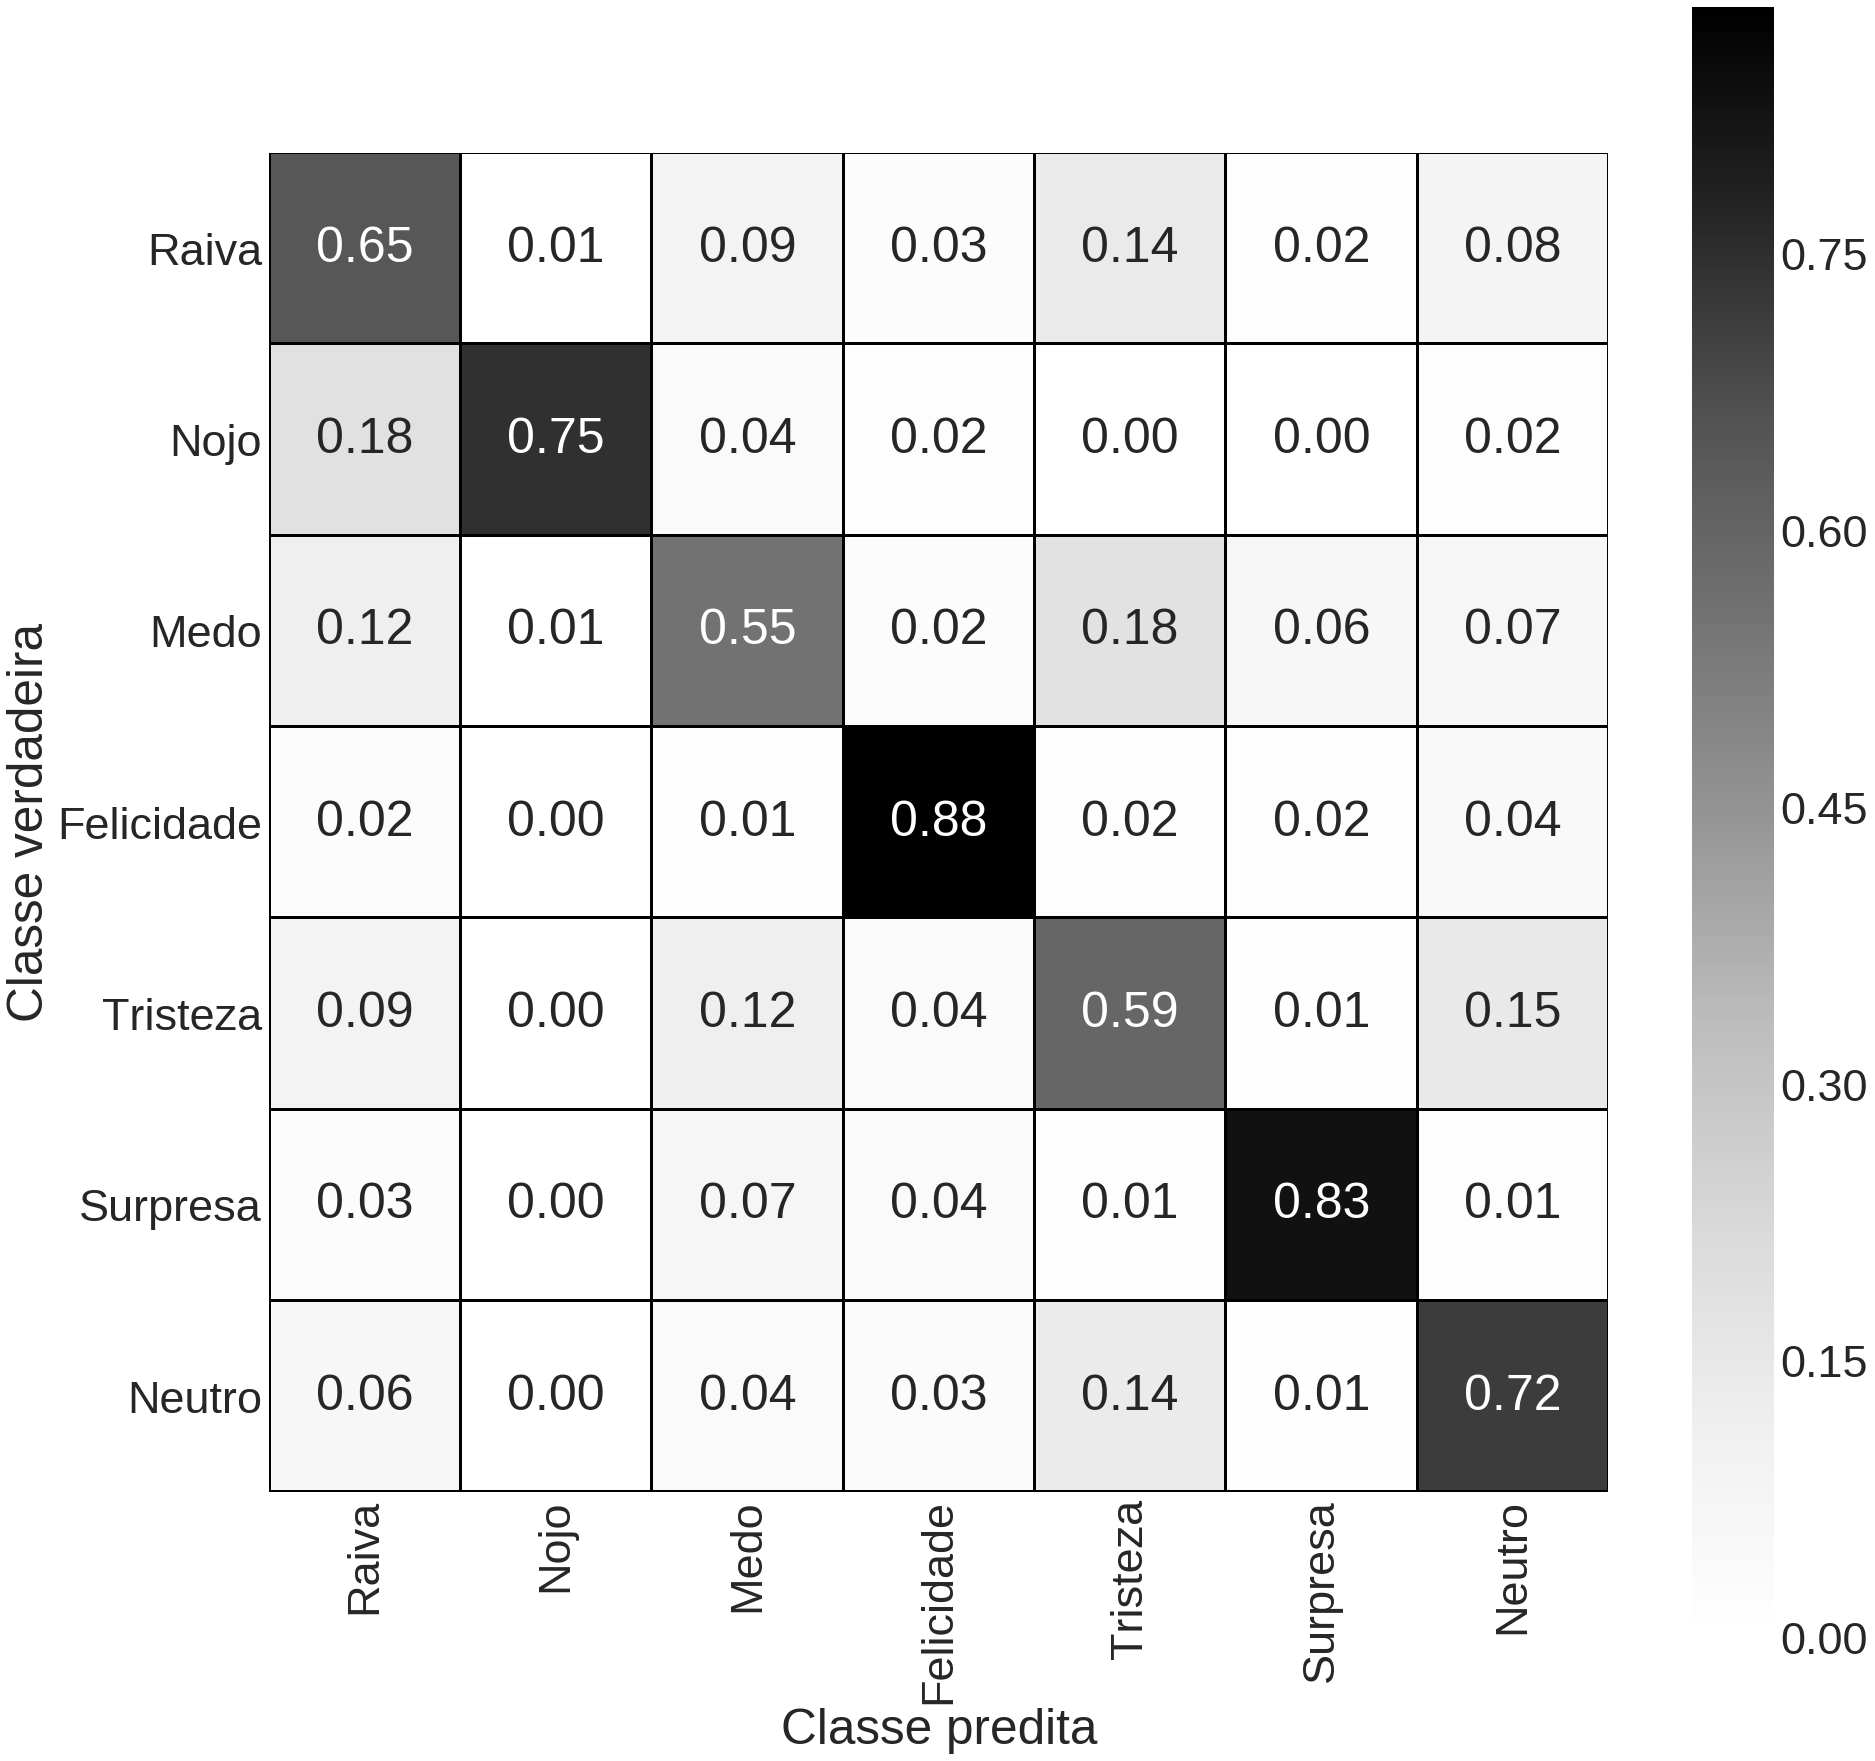
\includegraphics[width=9cm]{images/cm_emsemble.png}
    \caption{Matriz de Confusão do \emph{Ensemble} (CNN + \emph{XGBoost})}
    \label{fig:emsemble}
\end{figure}

Na diagonal principal da Matriz de Confusão Normalizada da Figura \ref{fig:emsemble} é possível observar os fundos das células mais escuros, que indica alta densidade de valores nessas células. E este comportamento evidencia a classificação correta de bastantes elementos do conjunto de teste, que apesar do desbalanceamento da base de dados apresentou bons resultados em expressões com poucas quantidades de elementos, como é o caso da expressão de nojo que obteve um dos melhores resultados \ref{fig:samples}, acompanhadas de surpresa e felicidade, com \textit{F1 Score} de 78\%, 83\%, e 89\% respectivamente. As classificações das outras expressões também apresentaram bons resultados, todas com \textit{F1 Score} maior ou igual a 58\%.

\begin{figure}[!htb]
    \centering
    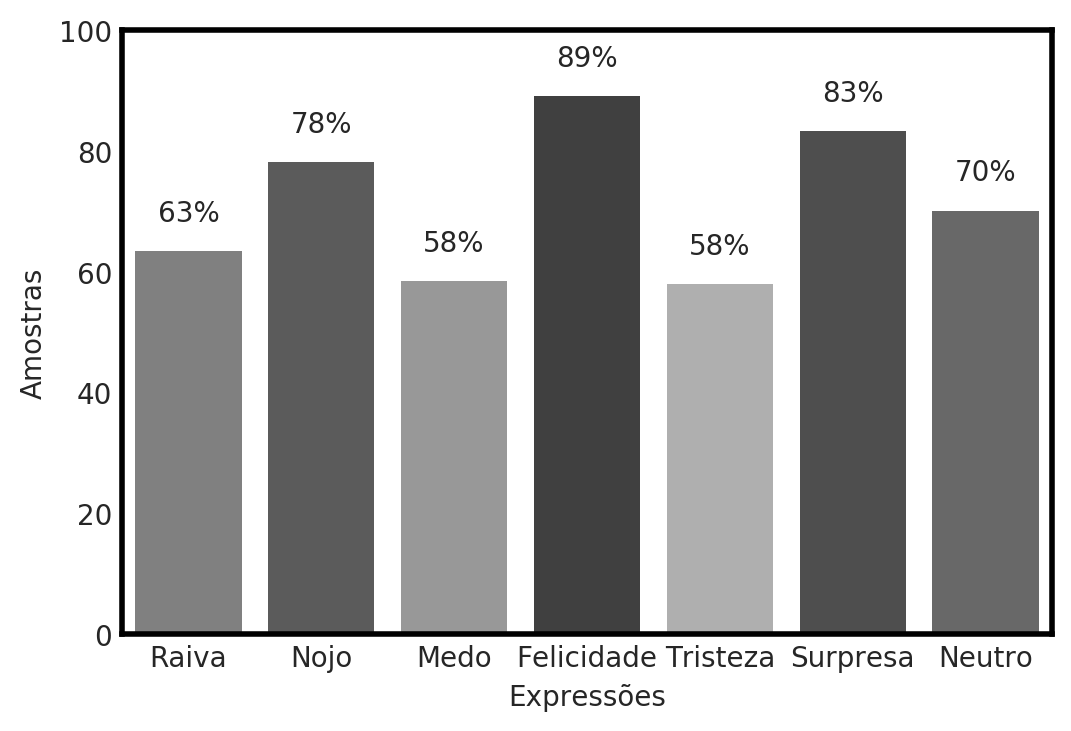
\includegraphics[width=8cm]{images/f1_bar.png}
    \caption{F1 Score por Expressão}
    \label{fig:f1_bar}
\end{figure}
